\section{1D 2G Homogeneous}
This problem is a simple version of a $k$-eigenvalue criticality problem using neutron diffusion.  While this problem is 1D, we use a 2D mesh to solve it by imposing reflecting boundary conditions on the top and bottom.  The governing PDE for this equation is
\begin{equation}
-\drv{}{x}D_g\drv{\phi_g}{x}+(\Sigma_{g,a}+\Sigma_{g,s})\phi_g = \sum_{g'}\sigma_{s}^{g'\to g}\phi_{g'} + \frac{\chi_{g}}{k}\sum_{g'}\nu_{g'}\sigma_{f,g'}\phi_{g'},\hspace{15pt} g\in[1,2],
\end{equation}
where $g$ denotes the energy group, $D$ is the group diffusion cross section; $\phi$ is the group flux, $x$ is the location within the problem; $\Sigma_a,\Sigma_s,\Sigma_f$ are the macroscopic absorption, scattering, and fission cross sections respectively; $k$ is the criticality factor eigenvalue and quantity of interest; and $\chi$ is the fraction of neutrons born into an energy group.  In this case, we consider only downscattering, and fission neutrons are only born into the high energy group ($\Sigma_s^{2\to1}=\chi_2=0$).

This problem does not have a convenient general analytic solution.  We can express the solver as
\begin{equation}
U(p;\theta) = k(p;\Sigma_{2,a}),
\end{equation}
where
\begin{equation}
p=(D_g,\Sigma_{1,a},\Sigma_{g,s},\nu_g,\Sigma_{g,f},\chi_g),\hspace{20pt}g\in[1,2].
\end{equation}
While $\phi_g(x)$ might also be considered a parameter, it is an output value solved simultaneously with $k$.

For this test code we consider $\theta=\Sigma_{2,a}$ in three possible normal distributions.  Evaluated at the distribution mean of $\theta$, we consider one each case where $k=(0.9,1.0,1.1)$, given by the distributions $\theta\in\mathcal{N}(0.09434,0.1), \theta\in\mathcal{N}(0.106695,0.1), \theta\in\mathcal{N}(0.08455,0.1)$ respectively.  A summary of all three cases is shown in Fig. \ref{1d_all}.  Tabular data for mean and variance convergence is in Tables \ref{tab:1dcrit} to \ref{tab:1dsub}, and the pdfs for each case are in Figs. \ref{fig:1dcrit} to \ref{fig:1dsub}.  It is important to note that the Monte Carlo sampling was restricted to values within 3 standard deviations of the mean; as such, the means and variances obtained directly through Monte Carlo sampling are not representative of the full uncertainty space.  This truncation of the distribution is enforced because without such a restriction, it is possible to sample physically untenable values for $\Sigma_{2,a}$, including negative values.

\begin{figure}[h!]
\centering
   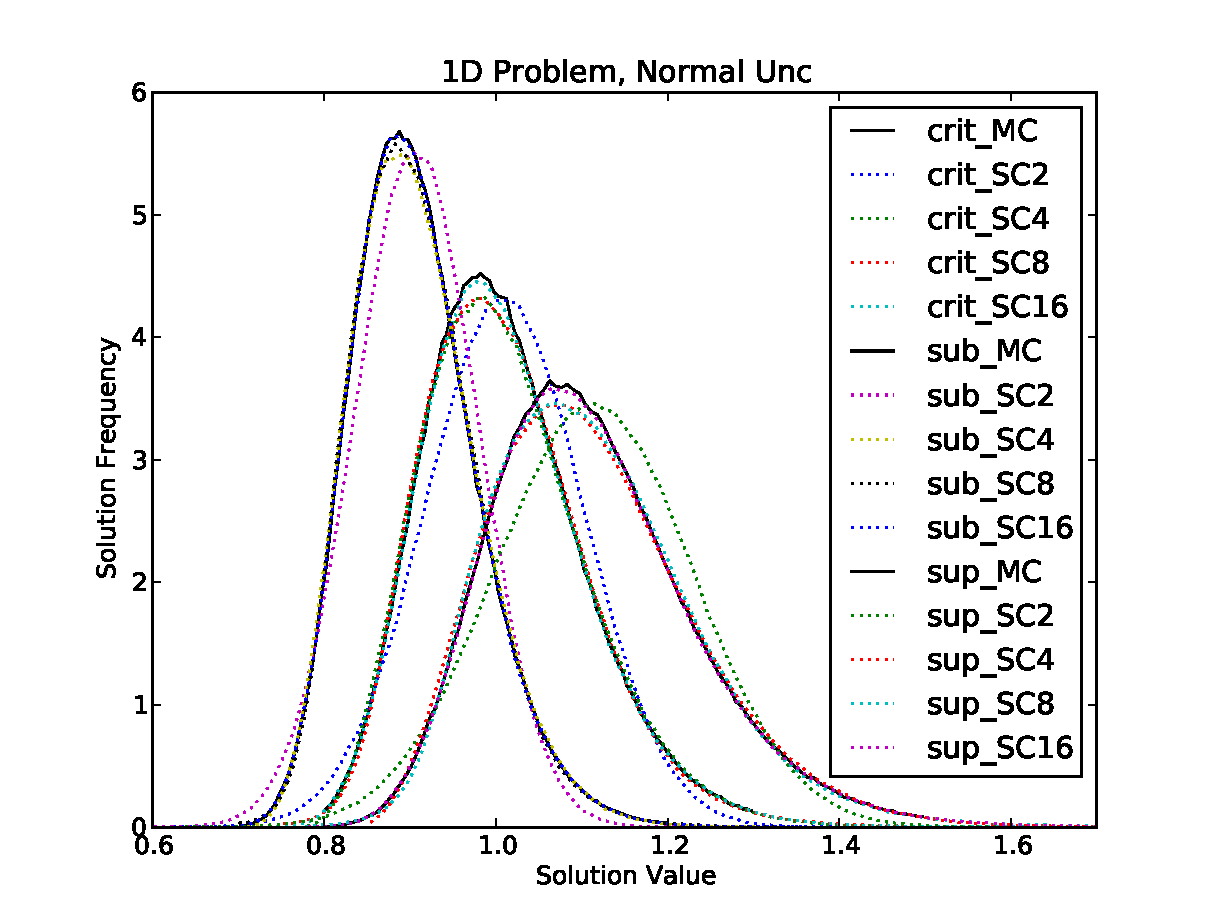
\includegraphics[width=.75\textwidth]{../graphics/1dall_normal_pdfs}
   \caption{Summary, 1D Criticality}
   \label{1d_all}
\end{figure}

\begin{table}
\begin{center}
\begin{tabular}{c c|l l}
type & runs/order & mean & variance \\ \hline
MC & $1\times10^6$ & 1.01023757498 & 0.0092547217648 \\
SC & 2 & 1.00999398244 & 0.00857615041851 \\
SC & 4 & 1.01022188926 & 0.00918078062636\\
SC & 8 & 1.010230418 & 0.0092238915176 \\
SC & 16 & 1.01023044508 & 0.00922009179288
\end{tabular}
\end{center}
\caption{Convergence of Mean, Variance for Critical Case}
\label{tab:1dcrit}
\end{table}

\begin{table}
\begin{center}
\begin{tabular}{c c|l l}
type & runs/order & mean & variance \\ \hline
MC & $1\times10^6$ & 1.11402940816 & 0.014621003 \\
SC & 2 & 1.11386614613 &0.0133637900516 \\
SC & 4 & 1.11426467694 &0.0145502163614 \\
SC & 8 & 1.114283758 &0.0146596758645 \\
SC & 16 & 1.11428385746 &0.0146501502189
\end{tabular}
\end{center}
\caption{Convergence of Mean, Variance for Supercritical Case}
\label{tab:1dsup}
\end{table}

\begin{table}
\begin{center}
\begin{tabular}{c c|l l}
type & runs/order & mean & variance \\ \hline
MC & $1\times10^6$ & 0.90705858894 &0.0055124462906   \\
SC & 2 & 0.906911426435 & 0.00521748368937  \\
SC & 4 & 0.907033407105 & 0.00550219402953 \\
SC & 8 & 0.907036892243 & 0.00551754177997  \\
SC & 16 & 0.907036898624 & 0.00551618720453
\end{tabular}
\end{center}
\caption{Convergence of Mean, Variance for Supercritical Case}
\label{tab:1dsub}
\end{table}

\begin{figure}[h!]
\centering
   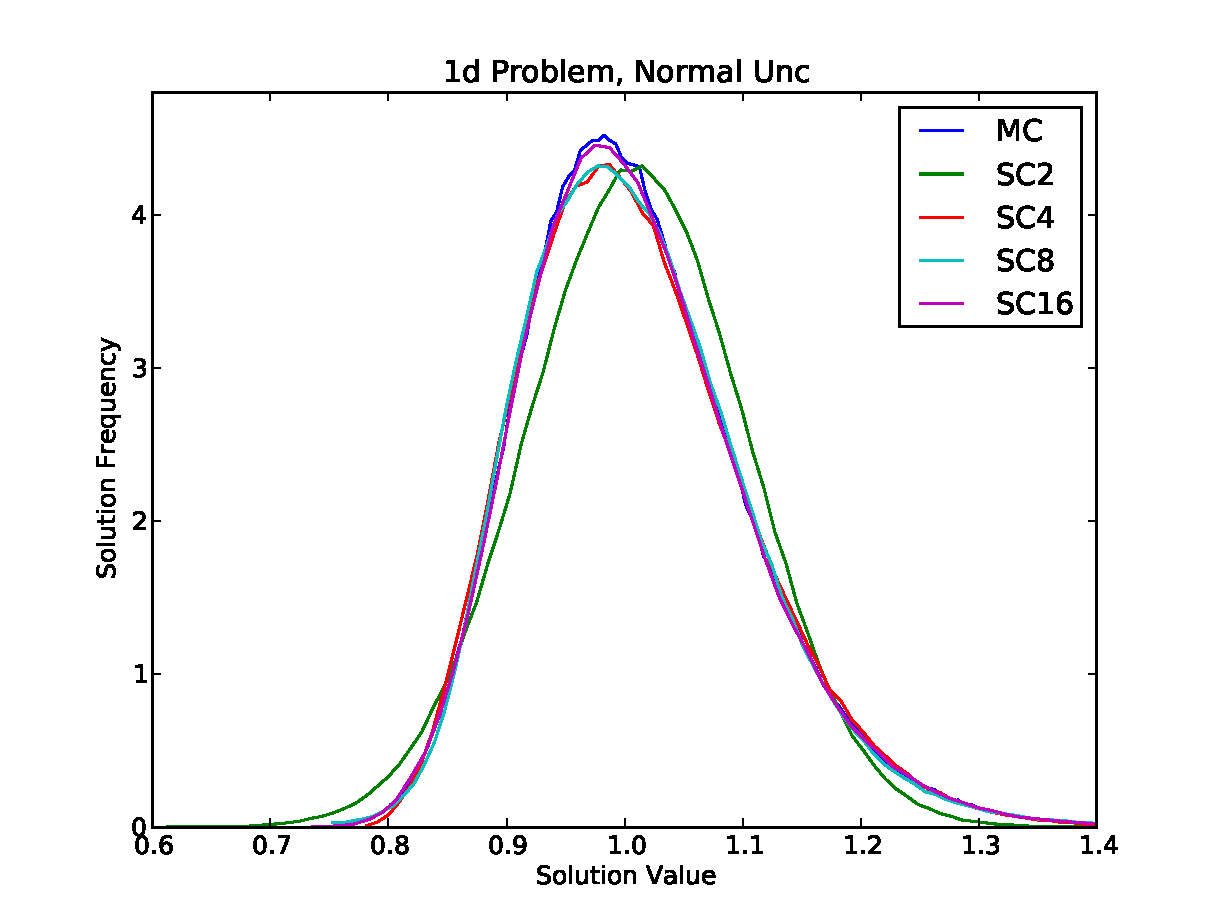
\includegraphics[width=.5\textwidth]{../graphics/1d_normal_pdfs}
   \caption{Solution PDF Convergence, 1D Critical Case}
   \label{fig:1dcrit}
\end{figure}

\begin{figure}[h!]
\centering
   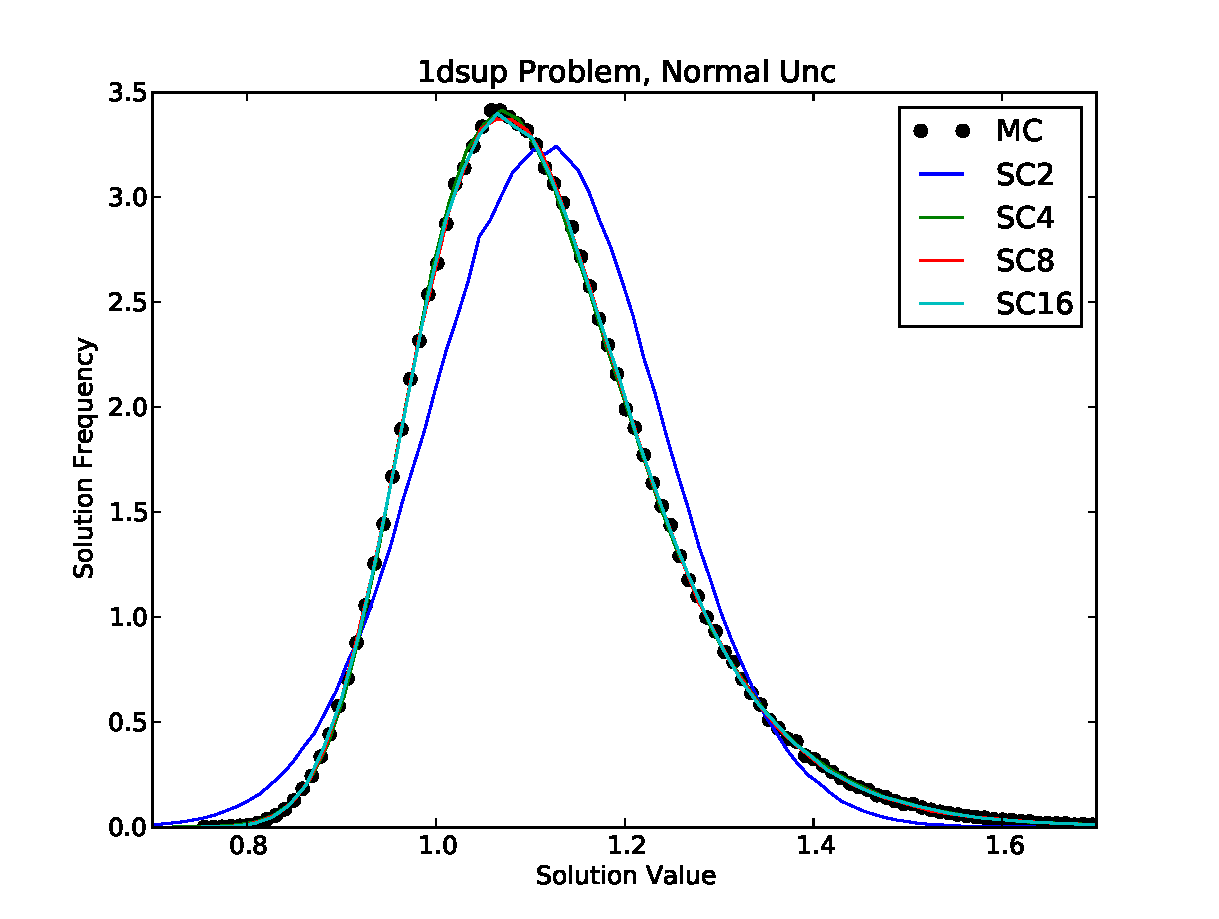
\includegraphics[width=.5\textwidth]{../graphics/1dsup_normal_pdfs}
   \caption{Solution PDF Convergence, 1D Supercritical Case}
      \label{fig:1dsup}
\end{figure}

\begin{figure}[h!]
\centering
   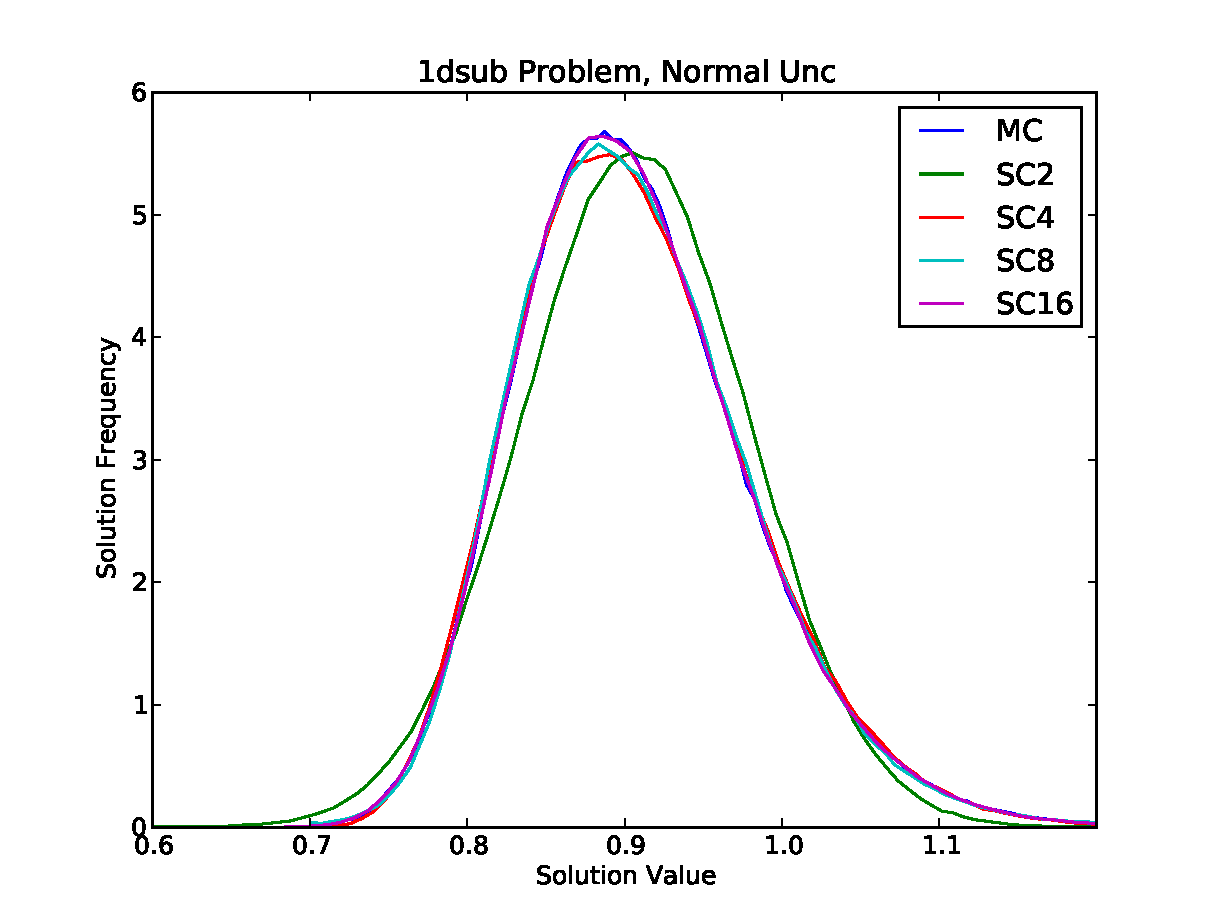
\includegraphics[width=0.5\textwidth]{../graphics/1dsub_normal_pdfs}
   \caption{Solution PDF Convergence, 1D Supercritical Case}
      \label{fig:1dsub}
\end{figure}


%
%\begin{figure}[h!]
%\centering
%   \includegraphics[width=\textwidth]{../graphics/}
%   \label{}
%   \caption{}
%\end{figure}
%\begin{table}
%\begin{center}
%\begin{tabular}{c c|l l| r}
%type & runs/order & mean & variance & run time (sec) \\ \hline
%MC & 1\times10^6 &  &  & \\
%SC & 2 & & & \\
%SC & 4 & & & \\
%SC & 8 & & & \\
%SC & 16 & & &
%\end{tabular}
%\end{center}
%\caption{}
%\label{}
%\end{table}
%
%\begin{figure}[h!]
%\centering
%   \includegraphics[width=\textwidth]{../graphics/}
%   \label{}
%   \caption{}
%\end{figure}
